%%
%%  Example paper
%%
%%

%%%%%%%%%%%%%%%%%% Usenix style %%%%%%%%%%%%%%%%%%%%%%%%%%%%%%%%%
\documentclass[10pt,twocolumn,a4paper]{article}
\usepackage{styles/usenix-style}

\author{Jakob Schmid}

%%%%%%%%%%%%%%%%%% Document %%%%%%%%%%%%%%%%%%%%%%%%%%%%%%%%%%%%%%%%%%%
% TODO: Change draft to final before submitting final version.
\usepackage[draft]{styles/ka-style}
\usepackage{cite,xspace,ifthen,graphicx,listings}

\usepackage[
   pdfauthor={Author},
   pdftitle={A Paper Template},
   pdfsubject={Paper Template},
   pdfkeywords={Papers, Templates}
]{hyperref}

\begin{document}

\title{Unikernel Linux (UKL)}

\newcommand{\todo}[1]{{\texttt{[#1]}}}
\newcommand{\code}[1]{{\tt \small{#1}}}

\maketitle
%\draftfooter

\begin{abstract}
  This report discusses Unikernel Linux (UKL), an approach to introduce a
  unikernel target into the Linux kernel.
  The specialized demand of cloud services has recently given rise
  to a resurgence of library operating systems in the form of unikernels.
  The authors of the UKL paper want to show that the Linux kernel can be
  modified to include the benefits of unikernels, while maintaining the
  ecosystem of applications and maintainers of Linux.
\end{abstract}

\section{Introduction}\label{sec:introduction}
  Modern cloud services are often highly specialised, to the point of a microservice, 
  where an applications is split up into a collection of loosely coupled services,
  that communicate through lightweight protocols and each only fullfill a single purpose.
  These services share a few key demands. They need to be able to communicate 
  efficiently with each other. Since they need to communicate with other services,
  they are exposed to the internet to some degree and thus should be as secure as possible.
  Due to the single purpose nature of the microservices they often execute as a single process.
  Lastly the image the service is executed with and the memory usage should be as small as possible.
  The services are often executed in a virtual machine on rented hardware, so lower requirements
  in memory and storage can improve the profitability of a service.
  These demands have caused a resurgence of research exploring the concept of a library OS and the
  emergence of unikernels. 

  In a library OS a target application is linked with a set of
  libraries that provide all the services a regular OS would usually provide.
  The resulting executable can then be deployed directly to hardware.
  In 2013 the term \textit{unikernel} was first introduced for library OSs
  for cloud services and deployment to virtual hardware \cite{madhavapeddy13}.

  Since then multiple unikernels have been created. Some are written from scratch like
  ClickOS \cite{martins2014} and Unikraft \cite{kuenzer21}.
  Others borrow code from an existing OS like Drawbridge \cite{porter11} 
  that uses code from Windows.

  UKL uses the Linux kernel as a base but tries to keep the changes minimal
  so that UKL can be maintained with the (general purpose) Linux kernel.
  

\section{Background}\label{sec:background}

\begin{figure}[htbp]
  \centering
  \fbox{\parbox{.8\columnwidth}{
      Here you can include a sample figure.  Use something like
      \begin{center}
        \code{$\backslash$includegraphics[scale=.8]\{template\}}
      \end{center}
      to include an encapsulated postscript figure.  The \emph{scale}
      argument can be used for scaling the picture, although it
      may scale the font incorrectly.
    }}
  \caption{Sample Figure}
  \label{fig:sample}
\end{figure}


\lstset{language=C, basicstyle=\ttfamily,
        string=[b]', showspaces=false, showtabs=false,
        caption={A sample code snippet}, captionpos=b}
\begin{lstlisting}
/* code snippet  */
while (!sleep)
	sleep++;
\end{lstlisting}

\begin{figure}[hbt]
\centering
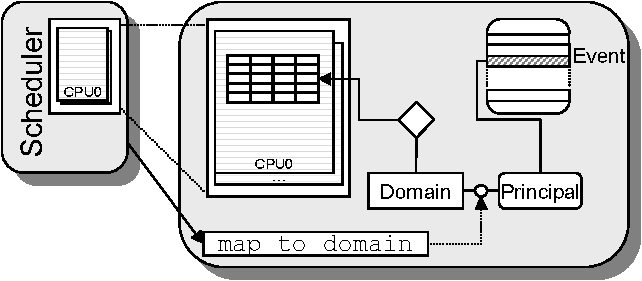
\includegraphics[scale=.7,clip]{fig/template}
\caption{Sample figure automatically from Windows prn.\label{plot:fig}}
\end{figure}

\section{Related Work}\label{sec:relwork} 

Works \cite{xen03virtualization} and \cite{pratt2005xaa} are relevant but
different.

\section{Approach}

\section{Conclusion}\label{sec:conclusion}

\bibliographystyle{abbrv}
\bibliography{template}
%\footnotesize
\end{document}
